\renewcommand*{\arraystretch}{1.1}

\subsection*{Interactive / short / 2}
\label{section:interactive-short-read-02}

% change \emph{} to use sans-serif font
\let\oldemph\emph
\renewcommand{\emph}[1]{{\footnotesize \sf #1}}

\renewcommand{\currentQueryCard}{2}
\marginpar{
	\raggedleft
	\vspace{0.22ex}

	\queryRefCard{interactive-short-read-01}{IS}{1}\\
	\queryRefCard{interactive-short-read-02}{IS}{2}\\
	\queryRefCard{interactive-short-read-03}{IS}{3}\\
	\queryRefCard{interactive-short-read-04}{IS}{4}\\
	\queryRefCard{interactive-short-read-05}{IS}{5}\\
	\queryRefCard{interactive-short-read-06}{IS}{6}\\
	\queryRefCard{interactive-short-read-07}{IS}{7}\\
}


\noindent\begin{tabularx}{\queryCardWidth}{|>{\queryPropertyCell}p{\queryPropertyCellWidth}|X|}
	\hline
	query & Interactive / short / 2 \\ \hline
%
	title & Person Recent Messages \\ \hline
%
	pattern & \multicolumn{1}{c|}{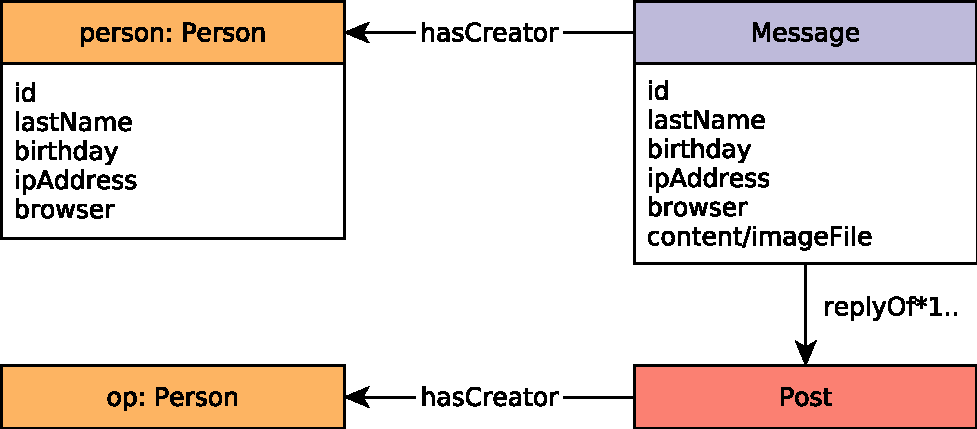
\includegraphics[scale=\patternscale,margin=0cm .2cm]{patterns/interactive-short-read-02}} \\ \hline
%
	desc. & Given a start Person, retrieve the last 10 Messages created by that
user. For each message, return that message, the original post in its
conversation, and the author of that post. If any of the Messages is a
Post, then the original Post will be the same Message, i.e.~that Message
will appear twice in that result.
 \\ \hline
%
	
		params &
		\innerCardVSpace{\begin{tabularx}{\attributeCardWidth}{|>{\paramNumberCell}c|>{\varNameCell}M|>{\typeCell}m{\typeWidth}|Y|} \hline
		$\mathsf{1}$ & Person.id
 & ID
 &  \\ \hline
		\end{tabularx}}\innerCardVSpace \\ \hline
	
%
	
		result &
		\innerCardVSpace{\begin{tabularx}{\attributeCardWidth}{|>{\resultNumberCell}c|>{\varNameCell}M|>{\typeCell}m{\typeWidth}|>{\resultOriginCell}c|Y|} \hline
		$\mathsf{1}$ & Message.id & 64-bit Integer & R &
				 \\ \hline
		$\mathsf{2}$ & Message.content or Post.imageFile & String & R &
				 \\ \hline
		$\mathsf{3}$ & Message.creationDate & DateTime & R &
				 \\ \hline
		$\mathsf{4}$ & Post.id or Comment-replyOf*-\textgreater{}Post.id & ID & R &
				 \\ \hline
		$\mathsf{5}$ & Post-hasCreator-\textgreater{}Person.id or
Comment-replyOf*-\textgreater{}Post-hasCreator-\textgreater{}Person.id & ID & R &
				 \\ \hline
		$\mathsf{6}$ & Post-hasCreator-\textgreater{}Person.firstName or
Comment-replyOf*-\textgreater{}Post-hasCreator-\textgreater{}Person.firstName & String & R &
				 \\ \hline
		$\mathsf{7}$ & Post-hasCreator-\textgreater{}Person.lastName or
Comment-replyOf*-\textgreater{}Post-hasCreator-\textgreater{}Person.lastName & String & R &
				 \\ \hline
		\end{tabularx}}\innerCardVSpace \\ \hline
	
%
	
		sort		&
		\innerCardVSpace{\begin{tabularx}{\attributeCardWidth}{|>{\sortNumberCell}c|>{\varNameCell}M|>{\directionCell}c|Y|} \hline
		$\mathsf{1}$ & Message.creationDate
 & $\desc
$ &  \\ \hline
		$\mathsf{2}$ & Message.id
 & $\desc
$ &  \\ \hline
		\end{tabularx}}\innerCardVSpace \\ \hline
	%
	%
	%
	%
\end{tabularx}
\queryCardVSpace

% change \emph back to the old one
\let\emph\oldemph